\begin{minipage}{.33\textwidth}
	\centering
	\textbf{reales Problem:}
	\resizebox{!}{.7\textwidth}{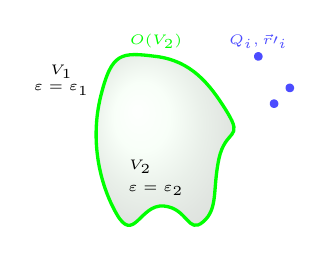
\begin{tikzpicture}[line width = 1.2pt, line join=round,>=stealth]
			\tiny;
		\filldraw [color=blue!70] (2.5,2.5) circle (1pt) node[above] {$Q_i, \vec{r}\prime _i$};
		\filldraw [color=blue!70] (2.9,2.1) circle (1pt);
		\filldraw [color=blue!70] (2.7,1.9) circle (1pt);
		% Ladungsdichte
		\coordinate (a) at (2.1,1.8);
		\coordinate (b) at (2,1.2);
		\coordinate (c) at (1.8,0.4);
		\coordinate (d) at (1.3,0.6);
		\coordinate (e) at (0.7,0.5);
		\coordinate (f) at (0.5,2);
		\coordinate (g) at (1.2,2.5);
		\shade[ball color=white!10!green!20,opacity=0.20] plot [smooth cycle, tension = 1] coordinates {(a) (b) (c) (d) (e) (f) (g)};
		\draw [color=green] plot [smooth cycle, tension = 1] coordinates {(a) (b) (c) (d) (e) (f) (g)} node [sloped, above] {$O(V_2)$};
		\draw(1,1.1) node {$V_2$};
		\draw(1.2,0.8) node{$\varepsilon=\varepsilon_2$};
		\draw(0,2.2) node[align=center] {$V_1$\\$\varepsilon=\varepsilon_1$};
	\end{tikzpicture}}
\end{minipage}
\begin{minipage}{.33\textwidth}
	\centering
	\textbf{Berechnung in} $V_1$:
	\resizebox{!}{.7\textwidth}{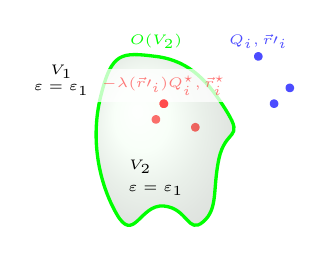
\begin{tikzpicture}[line width = 1.2pt, line join=round,>=stealth]
						\tiny;
		\filldraw [color=blue!70] (2.5,2.5) circle (1pt) node[above] {$Q_i, \vec{r}\prime _i$};
		\filldraw [color=blue!70] (2.9,2.1) circle (1pt);
		\filldraw [color=blue!70] (2.7,1.9) circle (1pt);
		\filldraw [color=red!70] (1.2,1.7) circle (1pt);
		\filldraw [color=red!70] (1.7,1.6) circle (1pt);
		% Ladungsdichte
		\coordinate (a) at (2.1,1.8);
		\coordinate (b) at (2,1.2);
		\coordinate (c) at (1.8,0.4);
		\coordinate (d) at (1.3,0.6);
		\coordinate (e) at (0.7,0.5);
		\coordinate (f) at (0.5,2);
		\coordinate (g) at (1.2,2.5);
		\shade[ball color=white!10!green!20,opacity=0.20] plot [smooth cycle, tension = 1] coordinates {(a) (b) (c) (d) (e) (f) (g)};
		\draw [color=green] plot [smooth cycle, tension = 1] coordinates {(a) (b) (c) (d) (e) (f) (g)} node [sloped, above] {$O(V_2)$};
		\draw(1,1.1) node {$V_2$};
		\draw(1.2,0.8) node{$\varepsilon=\varepsilon_1$};
		\draw(0,2.2) node[align=center] {$V_1$\\$\varepsilon=\varepsilon_1$};
		\filldraw [color=red!70] (1.3,1.9) circle (1pt) node[rectangle,fill=white,above,nearly opaque] {$-\lambda(\vec{r}\prime _i) Q^\star_i, \vec{r} ^\star_i$};
		\filldraw [color=red!70] (1.3,1.9) circle (1pt) ;
	\end{tikzpicture}}
\end{minipage}
\begin{minipage}{.33\textwidth}
	\centering
	\textbf{Berechnung in} $V_2$:
	\resizebox{!}{.7\textwidth}{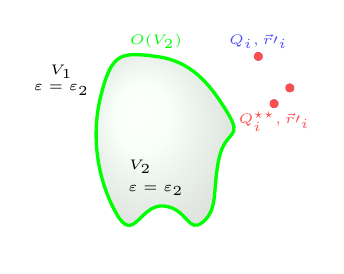
\begin{tikzpicture}[line width = 1.2pt, line join=round,>=stealth]
						\tiny;
		\filldraw [color=blue!70] (2.5,2.5) circle (1pt) node[above] {$Q_i, \vec{r}\prime _i$};
		\filldraw [color=blue!70] (2.9,2.1) circle (1pt);
		\filldraw [color=blue!70] (2.7,1.9) circle (1pt);
		\filldraw [color=red!70] (2.5,2.5) circle (1pt);
		\filldraw [color=red!70] (2.9,2.1) circle (1pt);
		\filldraw [color=red!70] (2.7,1.9) circle (1pt) node[below] {$Q_i^{\star\star}, \vec{r}\prime _i$};

		% Ladungsdichte
		\coordinate (a) at (2.1,1.8);
		\coordinate (b) at (2,1.2);
		\coordinate (c) at (1.8,0.4);
		\coordinate (d) at (1.3,0.6);
		\coordinate (e) at (0.7,0.5);
		\coordinate (f) at (0.5,2);
		\coordinate (g) at (1.2,2.5);
		\shade[ball color=white!10!green!20,opacity=0.20] plot [smooth cycle, tension = 1] coordinates {(a) (b) (c) (d) (e) (f) (g)};
		\draw [color=green] plot [smooth cycle, tension = 1] coordinates {(a) (b) (c) (d) (e) (f) (g)} node [sloped, above] {$O(V_2)$};
		\draw(1,1.1) node {$V_2$};
		\draw(1.2,0.8) node{$\varepsilon=\varepsilon_2$};
		\draw(0,2.2) node[align=center] {$V_1$\\$\varepsilon=\varepsilon_2$};
	\end{tikzpicture}}
\end{minipage}

